\documentclass{standalone}
\usepackage{tikz}
\usepackage{ctex,siunitx}
\setCJKmainfont{Noto Serif CJK SC}
\usepackage{tkz-euclide}
\usepackage{amsmath}
\usepackage{wasysym}
\usetikzlibrary{patterns, calc}
\usetikzlibrary {decorations.pathmorphing, decorations.pathreplacing, decorations.shapes,}
\begin{document}
\small
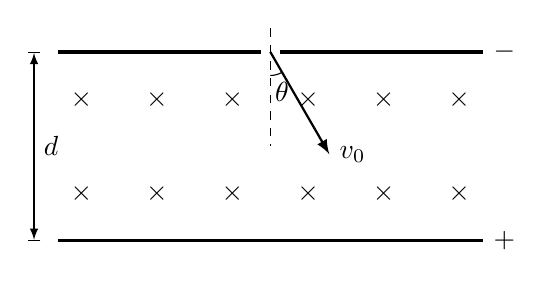
\begin{tikzpicture}[>=latex,scale=0.6]
  \draw[very thick](-4.5,2)--(-.2,2);
  \draw[very thick](.2,2)--(4.5,2)node[right]{$-$};
  \draw[very thick](-4.5,-2)--(4.5,-2)node[right]{$+$};
  \draw[dashed](0,2.5)--(0,0);
  \draw[->, thick](0,2)--+(-60:2.5)node[right]{$v_0$};
  \foreach \x in {.8,-.8,2.4,-2.4,4,-4}
  \foreach \y in {1,-1}
  {
    \node at (\x,\y){$\times$};
  }
  \draw[|<->|](-5,2)--(-5,-2)node[midway,right]{$d$};
  \draw(0,1.5) arc (-90:-60:.5)node[below]{$\theta$};
\end{tikzpicture}
\end{document}